\documentclass{report}

\usepackage[T2A]{fontenc}
\usepackage[utf8]{luainputenc}
\usepackage[english, russian]{babel}
\usepackage[pdftex]{hyperref}
\usepackage[14pt]{extsizes}
\usepackage{color}
\usepackage{geometry}
\usepackage{enumitem}
\usepackage{multirow}
\usepackage{graphicx}
\usepackage{indentfirst}
\usepackage{amsmath}
\usepackage{listings}
\usepackage{xcolor}
\usepackage{multicol}

%New colors defined below
\definecolor{codegreen}{rgb}{0,0.6,0}
\definecolor{codegray}{rgb}{0.5,0.5,0.5}
\definecolor{codepurple}{rgb}{0.58,0,0.82}
\definecolor{backcolour}{rgb}{0.95,0.95,0.92}

%Code listing style named "mystyle"
\lstdefinestyle{mystyle}{
  backgroundcolor=\color{backcolour},   commentstyle=\color{codegreen},
  keywordstyle=\color{magenta},
  numberstyle=\tiny\color{codegray},
  stringstyle=\color{codepurple},
  basicstyle=\ttfamily\footnotesize,
  breakatwhitespace=false,         
  breaklines=true,                 
  captionpos=b,                    
  keepspaces=true,                 
  numbers=left,                    
  numbersep=5pt,                  
  showspaces=false,                
  showstringspaces=false,
  showtabs=false,                  
  tabsize=2
}

%"mystyle" code listing set
\lstset{style=mystyle}

\geometry{a4paper,top=1cm,bottom=2cm,left=1cm,right=1cm}
\setlength{\parskip}{0.5cm}
\setlist{nolistsep, itemsep=0.3cm,parsep=0pt}

\begin{document}

\newpage

\par \textbf{6. Алгоритм обратного распространения ошибки на матричном языке.}
\par Прямой ход

\begin{align*}
& s_1 = w_1 + w_{11} x_1 + w_{12} x_2 \\
& s_2 = w_2 + w_{21} x_1 + w_{22} x_2 \\
& \begin{pmatrix} s_1 \\ s_2 \end{pmatrix} = \begin{pmatrix} w_1 \\ w_2 \end{pmatrix} + \begin{pmatrix} w_{11} & w_{12} \\ w_{21} & w_{22} \end{pmatrix} \begin{pmatrix} x_1 \\ x_2 \end{pmatrix} \\
& s = w + W x \\
& z = \sigma(s) \\
& \begin{pmatrix} t_1 \\ t_2 \end{pmatrix} = \begin{pmatrix} v_1 \\ v_2 \end{pmatrix} + \begin{pmatrix} v_{11} & v_{12} \\ v_{21} & v_{22} \end{pmatrix} \begin{pmatrix} z_1 \\ z_2 \end{pmatrix} \\
& t = v + V z \\
& R^{(i)} = logloss(g) \\
& g = softmax(t) \\
\end{align*}

\par $\sigma$ применяется покомпонентно.

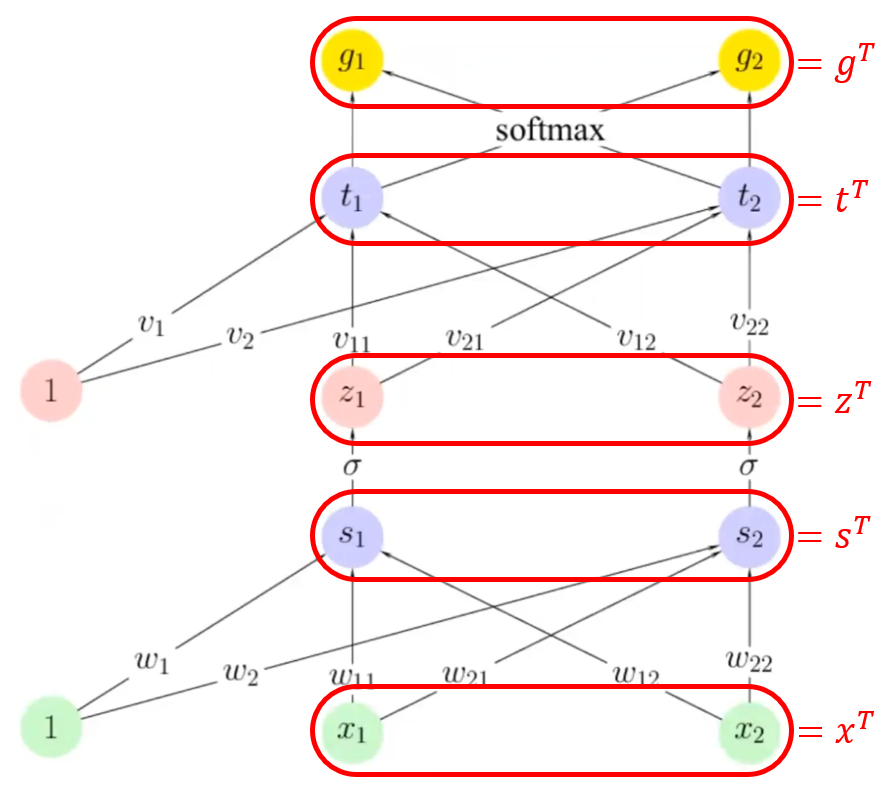
\includegraphics[width=0.6\textwidth]{exam/netletters.png}

\newpage
\par Обратный ход

\begin{multicols}{2}
\begin{align*}
    & \delta_t = \begin{pmatrix} \delta_{t1} \\ \delta_{t2} \end{pmatrix} = g - \begin{pmatrix} y_1^{(i)} \\ y_2^{(i)} \end{pmatrix} \\
    & \delta_{z1} = \delta_{t1} v_{11} + \delta_{t2} v_{21} \\
    & \delta_{z2} = \delta_{t1} v_{12} + \delta_{t2} v_{22} \\
    & (\delta_{z1}, \delta_{z2}) = (\delta_{t1}, \delta_{t2}) V \\
    & \delta_s = \delta_z \circ \sigma'(s) \\
    & \delta_x = \delta_s W = x \delta_{x_0} \\
\end{align*}
\columnbreak
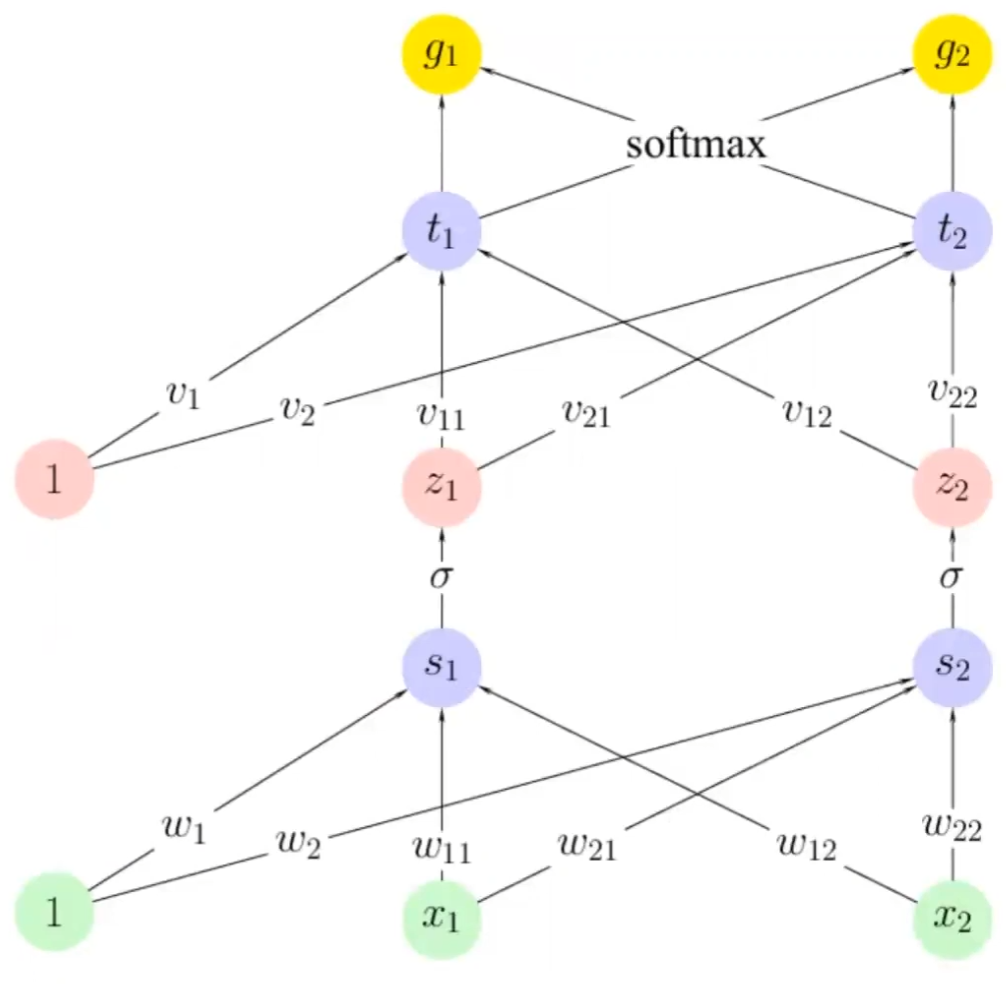
\includegraphics[width=0.36\textwidth]{exam/net.png}
\end{multicols}

\par $\circ$ обозначает покомпонентное применение.

\begin{align*}
& g = softmax(V(\sigma(Wx))) \\
& R^{(i)} = logloss(g) = \text{logloss}(\text{softmax}(V(\sigma(Wx)))) \\
& \text{Обозначим функцию logloss как } L \text{, функцию softmax как } g \text{:} \\
& R^{(i)} = L(g(V \cdot \sigma(Wx))) \\
& t(x) = V \cdot \sigma(Wx) \\
& z(x) = \sigma(Wx) \\
& s(x) = Wx \\
& R^{(i)} = L(g(t(x))) \\
& \text{Тогда с помощью матрично-векторного дифференцирования можно получить:} \\
& \frac{\partial R^{(i)}}{\partial x} = \frac{\partial L}{\partial g} \frac{\partial g}{\partial x} = \frac{\partial L}{\partial g} \frac{\partial g}{\partial t} \frac{\partial t}{\partial x} = \frac{\partial L}{\partial t} \frac{\partial t}{\partial x} = \frac{\partial L}{\partial t} \frac{\partial (V \cdot \sigma(s))}{\partial x} = \frac{\partial L}{\partial t} \frac{\partial (V \cdot \sigma(s))}{\partial \sigma} \frac{\partial \sigma}{\partial x} = \\
& = \frac{\partial R^{(i)}}{\partial t} \frac{\partial (V \cdot \sigma(Wx))}{\partial \sigma(Wx)} \frac{\partial \sigma(Wx)}{\partial Wx} \frac{\partial Wx}{\partial x} \\
& \frac{\partial (V \cdot \sigma(Ax))}{\partial \sigma(Wx)} = V,
  \frac{\partial \sigma(Wx)}{\partial Wx} = \text{diag}(\sigma'),
  \frac{\partial Wx}{\partial x} = W \\
& \frac{\partial R^{(i)}}{\partial t} = g - y = \delta_t \\
& \frac{\partial R^{(i)}}{\partial x} = (g - y) \cdot V \cdot \text{diag}(\sigma') \cdot W = \delta_x \\
& \frac{\partial R^{(i)}}{\partial W} = (g - y) \cdot V \cdot \text{diag}(\sigma') \cdot x = \delta_s \cdot x \\
& \frac{\partial R^{(i)}}{\partial V} = (g - y) \cdot \sigma(Wx) = \delta_t \cdot z
\end{align*}

\par Нас интересует вектор частных производных $R^{(i)}$ по каждой компоненте вектора $x$. Для этого находим частные производные и делаем шаг стохастического градиентного спуска. Шаг делается в пространстве весов (коэффициент $\gamma > 0$ - learning rate).

\begin{align*}
& W \leftarrow W - \gamma \frac{\partial R^{(i)}}{\partial W}, w \leftarrow w - \gamma \frac{\partial R^{(i)}}{\partial w}, \\
& V \leftarrow V - \gamma \frac{\partial R^{(i)}}{\partial V}, v \leftarrow v - \gamma \frac{\partial R^{(i)}}{\partial v} \\
\end{align*}

\end{document}
